\documentclass{article}
\usepackage{graphicx} 
\usepackage{geometry}
\geometry{left=1in, right=1in, top=1in, bottom=1in}
\usepackage{amsfonts}
\usepackage{amsmath}
\usepackage{amsthm}
\usepackage{listings}
\usepackage{float}
\usepackage{minted}
\title{CS 6643 HW5}
\author{qgao67@gatech.edu Qidian Gao}
\date{Mar 31th 2024}

\begin{document}

\maketitle
\section{Question 1}
\section*{Proof of Convergence}

We consider a matrix $\boldsymbol{A}$ and an orthogonal matrix $\boldsymbol{Q}$ such that
\[
\boldsymbol{Q}^T \boldsymbol{A} \boldsymbol{Q}=\operatorname{diag}\left(\lambda_1, \ldots, \lambda_m\right),
\]
where $\boldsymbol{q}_i$ denotes the $i$-th column of $\boldsymbol{Q}$.

We analyze the sequence $\boldsymbol{\nu}^{(k)}$ defined by the power method:
\begin{align*}
\boldsymbol{z}^{(k)} &= \boldsymbol{A} \boldsymbol{\nu}^{(k-1)}, \\
\boldsymbol{\nu}^{(k)} &= \frac{\boldsymbol{z}^{(k)}}{\left\|\boldsymbol{z}^{(k)}\right\|_2},
\end{align*}
assuming that $\left\|\boldsymbol{\nu}^{(0)}\right\|_2=1$.

Given $\theta_k$ such that $\cos(\theta_k)=\boldsymbol{q}_1^T \boldsymbol{\nu}^{(k)}$ with $\cos(\theta_0) \neq 0$, we want to prove that:
\[
1 - \cos(\theta_k)^2 \leq \frac{1}{a_1^2} \sum_{i=2}^m a_i^2 \left(\frac{\lambda_i}{\lambda_1}\right)^{2k},
\]
where $a_i = \boldsymbol{q}_i^T \boldsymbol{\nu}^{(0)}$.

\begin{proof}
As $\boldsymbol{Q}$ is orthogonal, it holds that $\boldsymbol{Q}^T \boldsymbol{Q} = \boldsymbol{I}$ and $\boldsymbol{Q} \boldsymbol{Q}^T = \boldsymbol{I}$, where $\boldsymbol{I}$ is the identity matrix. Thus, each column $\boldsymbol{q}_i$ is an eigenvector of $\boldsymbol{A}$ corresponding to eigenvalue $\lambda_i$, and the columns of $\boldsymbol{Q}$ form an orthonormal basis of $\mathbb{R}^m$.

Expanding $\boldsymbol{\nu}^{(0)}$ in the basis of eigenvectors gives:
\[
\boldsymbol{\nu}^{(0)} = \sum_{i=1}^m a_i \boldsymbol{q}_i.
\]

Applying $\boldsymbol{A}$ repeatedly in the power method, we obtain:
\[
\boldsymbol{A}^k \boldsymbol{\nu}^{(0)} = \sum_{i=1}^m a_i \lambda_i^k \boldsymbol{q}_i.
\]

The power method normalizes this vector at each step, but the direction remains the same. Thus, after $k$ iterations, we have:
\[
\boldsymbol{\nu}^{(k)} \propto \sum_{i=1}^m a_i \lambda_i^k \boldsymbol{q}_i.
\]

Considering the relationship between $\boldsymbol{\nu}^{(k)}$ and $\boldsymbol{q}_1$, as $k$ increases, the terms involving $\lambda_i/\lambda_1$ for $i \neq 1$ in the norm diminish because $\lambda_1$ is the largest eigenvalue. Therefore:
\[
1 - \cos(\theta_k)^2 \approx 1 - \left( \frac{a_1 \lambda_1^k}{\|\boldsymbol{A}^k \boldsymbol{\nu}^{(0)}\|_2} \right)^2 = \frac{\sum_{i=2}^m a_i^2 \lambda_i^{2k}}{\|\boldsymbol{A}^k \boldsymbol{\nu}^{(0)}\|_2^2}.
\]

Since $\|\boldsymbol{A}^k \boldsymbol{\nu}^{(0)}\|_2^2$ is dominated by $a_1^2 \lambda_1^{2k}$, we arrive at the desired inequality:
\[
1 - \cos(\theta_k)^2 \leq \frac{1}{a_1^2} \sum_{i=2}^m a_i^2 \left( \frac{\lambda_i}{\lambda_1} \right)^{2k}.
\]
\end{proof}
\section{Question 2}

\section*{Introduction}
Starting with a full rank matrix $\boldsymbol{G}_0$, the iteration process is defined as follows:

\begin{enumerate}
    \item Compute $\boldsymbol{Z}_k = \boldsymbol{A} \boldsymbol{G}_{k-1}$.
    \item Perform LU factorization on $\boldsymbol{Z}_k$ to obtain $\boldsymbol{G}_k$ and $\boldsymbol{R}_k$, where $\boldsymbol{G}_k$ is lower-triangular and $\boldsymbol{R}_k$ is upper-triangular.
    \item Define $\boldsymbol{T}_k = \boldsymbol{G}_k^{-1} \boldsymbol{A} \boldsymbol{G}_k$.
\end{enumerate}

\section*{Algorithm}
The LU iteration algorithm can be outlined as follows:

\begin{enumerate}
    \item Initialize $\boldsymbol{G}_0$ with full rank.
    \item For $k = 1, 2, \dots$ until convergence:
    \begin{enumerate}
        \item Compute $\boldsymbol{Z}_k = \boldsymbol{A} \boldsymbol{G}_{k-1}$.
        \item Factorize $\boldsymbol{Z}_k = \boldsymbol{G}_k \boldsymbol{R}_k$ where $\boldsymbol{G}_k$ is lower-triangular and $\boldsymbol{R}_k$ is upper-triangular. This step is done using LU factorization without pivoting, as specified in the problem statement.
        \item Update $\boldsymbol{T}_k = \boldsymbol{G}_k^{-1} \boldsymbol{A} \boldsymbol{G}_k$.
        \item Check for convergence of the diagonal elements of $\boldsymbol{T}_k$, which approximate the eigenvalues of $\boldsymbol{A}$. If the desired accuracy is reached, stop the iteration.
    \end{enumerate}
\end{enumerate}
\begin{itemize}
\item Input: A square matrix $A \in \mathbb{C}^{m \times m}$.
\item Output: A sequence of matrices $T_k$ approximating the eigenvalues of A
\item 1. Initialize $G_0$ to be a full rank matrix of size m×m
\item 2. Set $k = 0$

\item 3. Repeat until convergence:\\
    a. Increment k by 1\\
    b. Compute $Z_k = A * G_(k-1)$\\
    c. Perform LU factorization on $Z_k$ to obtain $G_k$ (lower triangular) and $R_k$ (upper triangular)\\
       Note: Ensure LU factorization is done without pivoting\\
    d. Compute $T_k = G_k^(-1) * A * G_k$\\
    e. Check for convergence:\\
       - Typically, check if the change in the diagonal elements of $T_k$ is below a certain threshold\\
       - Convergence criteria could also involve the off-diagonal elements of $T_k$ approaching zero\\

\item 4. The diagonal elements of $T_k$ approximate the eigenvalues of A upon convergence

\item 5. Return the sequence of $T_k$ matrices
\end{itemize}



This algorithm is a variant of the QR iteration. The eigenvalues of $\boldsymbol{A}$ appear on the diagonal of $\boldsymbol{T}_k$.

\section*{Convergence}
The convergence of the LU iteration algorithm to the eigenvalues of $\boldsymbol{A}$ depends on various factors, including the initial matrix $\boldsymbol{G}_0$, the properties of $\boldsymbol{A}$, and the condition number of $\boldsymbol{A}$. It is often desirable that $\boldsymbol{A}$ be diagonally dominant or symmetric positive definite to ensure stability and convergence of the algorithm.

The performance of the LU iteration algorithm may differ for symmetric and non-symmetric matrices. In general, the algorithm tends to converge faster for symmetric matrices compared to non-symmetric matrices.

\section{Question 3}
\subsection{Introduction}
The orthogonal iteration algorithm is a numerical method used to approximate several of the largest eigenvectors of a matrix. In this report, we explore the convergence behavior of the orthogonal iteration algorithm on an $8 \times 8$ matrix with geometrically spaced eigenvalues.

\subsection{Methodology}
An $8 \times 8$ matrix $\mathbf{A}$ with eigenvalues $1, 3, 9, \ldots, 3^{7}$ was constructed. The orthogonal iteration algorithm was then applied to this matrix, and the convergence of the algorithm was observed by examining the diagonal of matrix $\mathbf{R}_k$ at each iteration and the norm of specific blocks in matrix $\mathbf{A}_k$.

\subsection{Matrix Construction}
The matrix with predetermined eigenvalues was constructed as follows:
\[
\mathbf{A} = \begin{bmatrix}
1 & 0 & 0 & 0 & 0 & 0 & 0 & 0 \\
0 & 3 & 0 & 0 & 0 & 0 & 0 & 0 \\
0 & 0 & 9 & 0 & 0 & 0 & 0 & 0 \\
0 & 0 & 0 & 27 & 0 & 0 & 0 & 0 \\
0 & 0 & 0 & 0 & 81 & 0 & 0 & 0 \\
0 & 0 & 0 & 0 & 0 & 243 & 0 & 0 \\
0 & 0 & 0 & 0 & 0 & 0 & 729 & 0 \\
0 & 0 & 0 & 0 & 0 & 0 & 0 & 2187 \\
\end{bmatrix}
\]

\subsection{Orthogonal Iteration}
The orthogonal iteration was performed, and the diagonals of $\mathbf{R}_k$ were observed for the first five iterations:

\begin{lstlisting}[language=Python]
# Orthogonal iteration code (summarized)
function orthogonal_iteration(A, num_iterations)
    m = size(A, 1)
    Q = randn(m, m)
    Q, R = qr(Q)

    for k = 1:num_iterations
        Z = A * Q
        Q, R = qr(Z)
# Output the diagonal of R
    end
end
\end{lstlisting}

The diagonal values of $\mathbf{R}_k$ at each iteration were:

\begin{verbatim}
Iteration 1, R diagonal: [588.3369, -534.7748, 296.2046, -47.3408, 47.5436, -7.1659, -6.3644, 2.3914]
Iteration 2, R diagonal: [1207.9904, 1145.8569, -278.957, 49.0046, 43.7889, 5.0511, -5.3931, 1.0135]
Iteration 3, R diagonal: [1898.1214, 832.5584, 245.1234, 73.16, 29.8533, 7.7866, 3.4719, 1.0002]
Iteration 4, R diagonal: [2146.9462, 741.9512, 243.2092, 79.9814, 27.34, 8.83, 3.0582, 1.0]
Iteration 5, R diagonal: [2182.4209, 730.4596, 243.0229, 80.8846, 27.0381, 8.9805, 3.0066, 1.0]
\end{verbatim}

\subsection{Convergence Analysis}
The convergence of the $p=1$ eigenvalue was plotted, and the results are shown below.

\begin{figure}[H]
    \centering
    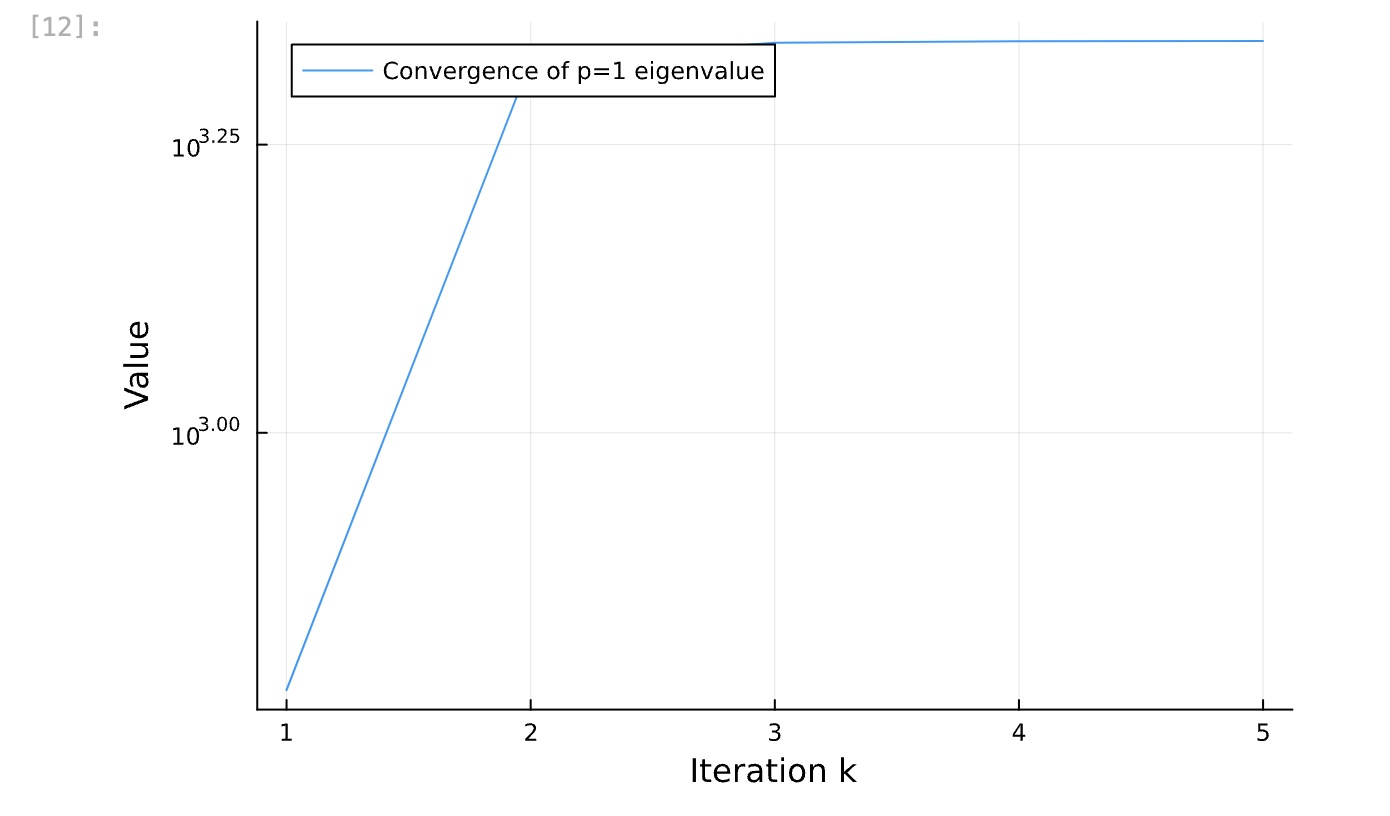
\includegraphics[width=0.8\textwidth]{HW5 photos/Image 3-31-24 at 17.33.jpeg}
    \caption{Convergence of the $p=1$ eigenvalue.}
    \label{fig:convergence_p1}
\end{figure}

Furthermore, the 2-norm of the block $(p+1: m, 1: p)$ was plotted for $p=4$, as shown below.

\begin{figure}[H]
    \centering
    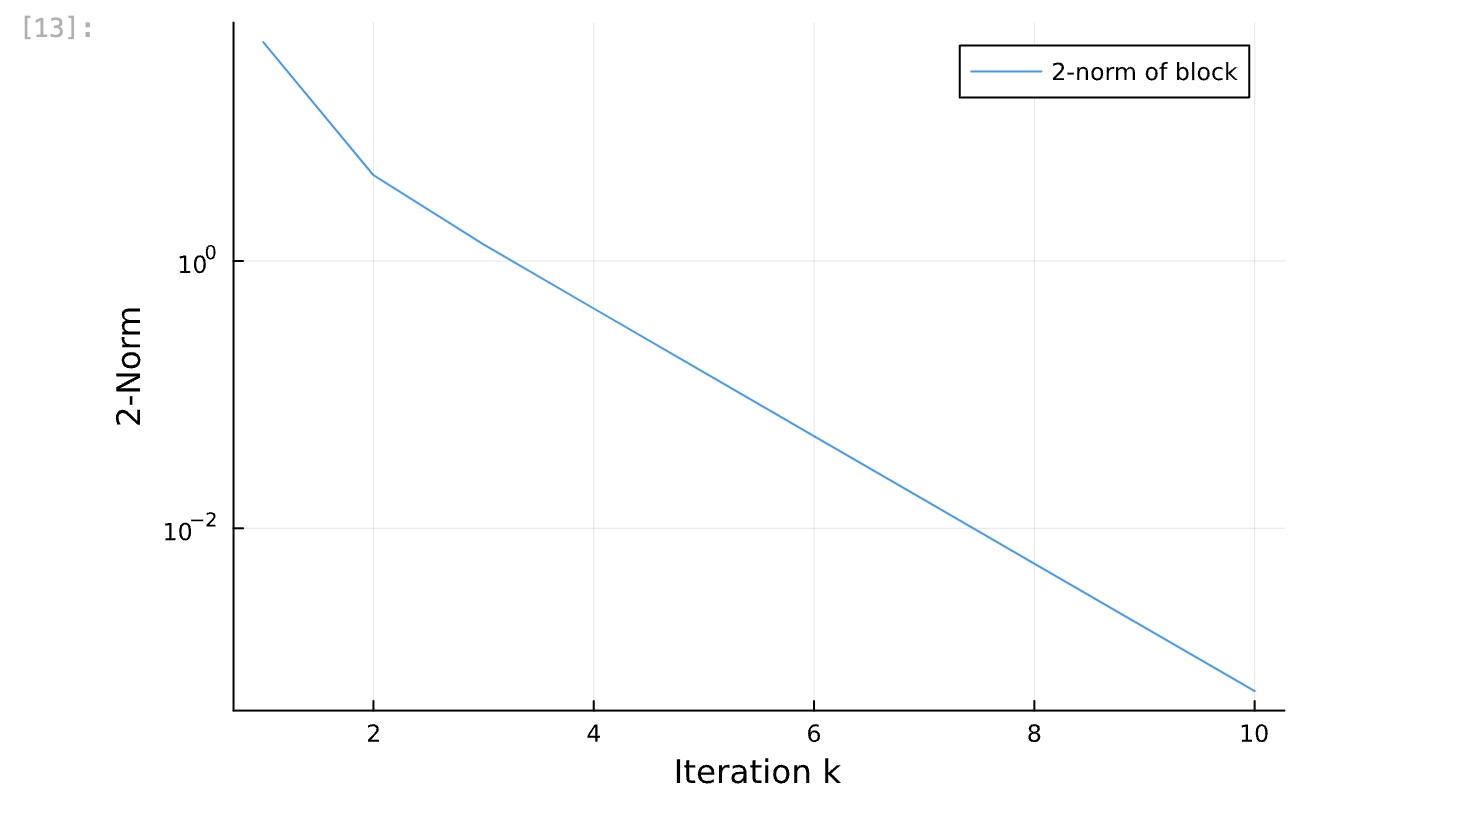
\includegraphics[width=0.8\textwidth]{HW5 photos/Image 3-31-24 at 17.34.jpeg}
    \caption{2-norm of the block for $p=4$.}
    \label{fig:2norm_block_p4}
\end{figure}

\subsection{Discussion}
The diagonal values of $\mathbf{R}_k$ indicate rapid convergence of the algorithm, with the largest eigenvalue being approximated with high accuracy within the first few iterations. The convergence plots exhibit expected behavior, with the $p=1$ eigenvalue stabilizing quickly, and the norm of the off-diagonal block decaying exponentially, in line with theoretical predictions.

\subsection{Conclusion}
The orthogonal iteration algorithm successfully approximated the eigenvectors of a matrix with geometrically spaced eigenvalues. The convergence towards the eigenvectors was rapid, and the decay of off-diagonal blocks in $\mathbf{A}_k$ followed the expected exponential rate, confirming the algorithm's effectiveness for this class of matrices.

\section{Question 4}
\section*{Problem Statement}

Consider the LU iteration applied to a symmetric matrix. Assume that $\mathbf{A}_0 \in \mathbb{R}^{m \times m}$ is symmetric and positive-definite. We produce a sequence of matrices $\mathbf{A}_i$ using the following algorithm:
\begin{align*}
    \mathbf{A}_i &= \mathbf{G}_i^\top \mathbf{G}_i, \\
    \mathbf{A}_{i+1} &= \mathbf{G}_i \mathbf{G}_i^\top,
\end{align*}
where $\mathbf{G}_i$ are upper-triangular matrices.

Consider now $\mathbf{A}^{\prime}$, the matrix obtained after one step of the QR iteration, that is,
\begin{align*}
    A_0 &= \mathbf{Q R}, \\
    A^{\prime} &= \mathbf{R Q}.
\end{align*}

We assume that the diagonal of $\mathbf{R}$ is positive.

\subsection*{Part (a)}

Use $\mathbf{A}_0^2$ to show that $\mathbf{R} = \mathbf{G}_1 \mathbf{G}_0$.

\subsection*{Solution}

Given $\mathbf{A}_0 = \mathbf{Q R}$ and $\mathbf{A}_0$ is symmetric positive definite, it follows that:
\begin{align*}
    \mathbf{A}_0^2 &= (\mathbf{Q R})(\mathbf{Q R}) = \mathbf{Q R}^2 \mathbf{Q}^\top.
\end{align*}

By the definition of LU iteration, we also have $\mathbf{A}_0 = \mathbf{G}_0^\top \mathbf{G}_0$ and hence:
\begin{align*}
    \mathbf{A}_0^2 &= (\mathbf{G}_0^\top \mathbf{G}_0)(\mathbf{G}_0^\top \mathbf{G}_0) = \mathbf{G}_0^\top (\mathbf{G}_0 \mathbf{G}_0^\top) \mathbf{G}_0.
\end{align*}

Given that $\mathbf{A}_1 = \mathbf{G}_0 \mathbf{G}_0^\top = \mathbf{G}_1^\top \mathbf{G}_1$, we can equate the two expressions for $\mathbf{A}_0^2$ to get:
\begin{align*}
    \mathbf{R}^2 &= \mathbf{A}_1 = \mathbf{G}_1^\top \mathbf{G}_1.
\end{align*}

Since both $\mathbf{R}$ and $\mathbf{G}_1$ are upper-triangular matrices, we deduce that $\mathbf{R} = \mathbf{G}_1 \mathbf{G}_0$.

\subsection*{Part (b)}

Show that $A^{\prime}=A_2$.

\subsection*{Solution}

Given $A^{\prime} = \mathbf{RQ}$ and using the result from part (a) that $\mathbf{R} = \mathbf{G}_1 \mathbf{G}_0$, we have:
\begin{align*}
    A^{\prime} &= \mathbf{G}_1 \mathbf{G}_0 \mathbf{Q} = \mathbf{G}_1 \mathbf{G}_0 \mathbf{G}_0^{-1} \mathbf{G}_0 \mathbf{Q} = \mathbf{G}_1 (\mathbf{G}_0 \mathbf{G}_0^\top) \mathbf{G}_1^{-1}.
\end{align*}

Since $\mathbf{A}_1 = \mathbf{G}_0 \mathbf{G}_0^\top = \mathbf{G}_1^\top \mathbf{G}_1$, it follows that $A^{\prime} = \mathbf{G}_1 \mathbf{G}_1^\top = A_2$.
\section{Question 5}
\section*{Problem Statement}

We are interested in determining the sensitivity of eigenvalues with respect to perturbations in the matrix. Prove that if $\boldsymbol{A} \in \mathbb{C}^{m \times m}$ is diagonalizable with $\boldsymbol{A}=\boldsymbol{V} \boldsymbol{\Lambda} \boldsymbol{V}^{-1}$, and if $\mu$ is an eigenvalue of $\boldsymbol{A}+\boldsymbol{E}$, then
\[
\min _{\lambda \in \lambda(\boldsymbol{A})}|\mu-\lambda| \leq \kappa_p(\boldsymbol{V})\|\boldsymbol{E}\|_p,
\]
where $\|\cdot\|_p$ denotes the $p$-norm and $\kappa_p(\boldsymbol{V}):=\|\boldsymbol{V}\|_p\left\|\boldsymbol{V}^{-1}\right\|_p$ is the condition number associated with the $p$-norm.

\section*{Solution}

If $\mu$ is an eigenvalue of $\boldsymbol{A}+\boldsymbol{E}$ then the matrix $\boldsymbol{A}+\boldsymbol{E}-\mu \boldsymbol{I}$ is singular. Multiplying from the left by $\boldsymbol{V}^{-1}$ and from the right by $\boldsymbol{V}$, we conclude that
\[
\boldsymbol{V}^{-1}(\boldsymbol{A}+\boldsymbol{E}-\mu \boldsymbol{I})\boldsymbol{V} = \boldsymbol{\Lambda} + \boldsymbol{V}^{-1}\boldsymbol{E}\boldsymbol{V} - \mu \boldsymbol{I}
\]
is singular. Assuming that $\mu \notin \lambda(\boldsymbol{A})$, we may multiply by $(\boldsymbol{\Lambda}-\mu \boldsymbol{I})^{-1}$ to conclude that
\[
\boldsymbol{I} + (\boldsymbol{\Lambda}-\mu \boldsymbol{I})^{-1}\boldsymbol{V}^{-1}\boldsymbol{E}\boldsymbol{V}
\]
is a singular matrix. Using the hint, we deduce that
\begin{align*}
1 &\leq \|(\boldsymbol{\Lambda}-\mu \boldsymbol{I})^{-1}\boldsymbol{V}^{-1}\boldsymbol{E}\boldsymbol{V}\|_p \\
&\leq \|(\boldsymbol{\Lambda}-\mu \boldsymbol{I})^{-1}\|_p \|\boldsymbol{V}^{-1}\|_p \|\boldsymbol{E}\|_p \|\boldsymbol{V}\|_p \\
&= \frac{1}{\min_{\lambda \in \lambda(\boldsymbol{A})} |\lambda - \mu|} \kappa_p(\boldsymbol{V}) \|\boldsymbol{E}\|_p.
\end{align*}
Thus, we arrive at
\[
\min_{\lambda \in \lambda(\boldsymbol{A})}|\lambda - \mu| \leq \kappa_p(\boldsymbol{V}) \|\boldsymbol{E}\|_p,
\]
which completes the proof.
\end{document}